\chapter{Background}
\label{chap:background}

\Ac{io} devices interact with the \acs{cpu} via interrupts, registers and shared
memory. We provide an overview of how these communication primitives work with
\acp{iommu} in context of network environments in the following sections,
focusing on \acs{pcie}, \acsp{nic}, \acsp{iommu} on Linux, and \acs{sriov}.


\section{Overview}
\label{sec:overview}

\begin{figure}[!b]
    \centering
    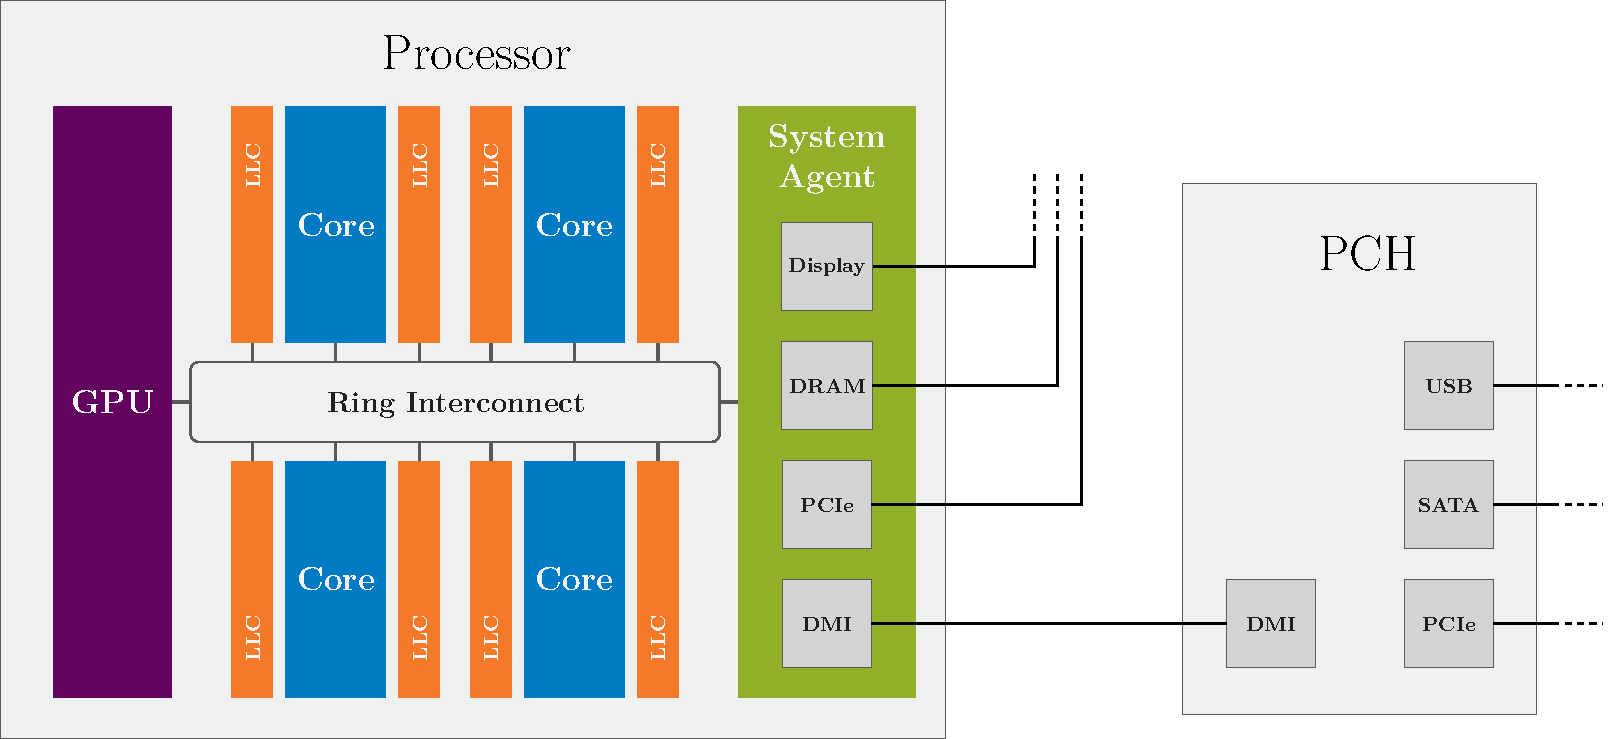
\includegraphics[width=0.8\textwidth]{figures/cpu-and-pch}
    \caption{Processor and Platform Controller Hub (PCH) on an Intel system.}
    \label{fig:pch}
\end{figure}

On modern systems, peripherals, processor and main memory are interconnected via
a wide set of connection standards and protocols. Devices are either directly
attached to the \ac{cpu} via \ac{pcie} or to an \acs{io} hub known as Platform
Controller Hub~(Intel) or chipset~(AMD). Direct connections are preferred for
\ac{io} devices with high performance requirements such as video cards or NVMe
controllers. On enterprise hardware, e.g., servers, most \ac{pcie} devices are
directly attached to the \ac{cpu}, whereas the \ac{io} hub is connected to
slower peripherals like on-board Gigabit network cards. On consumer hardware,
more devices are usually attached to the \ac{io} hub. The \ac{io} hub resides on
a separate chip and is connected to the \ac{cpu} via Direct Media Interface
(Intel) or Unified Media Interface (AMD). \Cref{fig:pch} illustrates the
relationship between \ac{cpu}, \ac{io} hub and peripherals. Conceptually, system
agent and Platform Controller Hub (PCH) depicted in \Cref{fig:pch} are
successors of northbridge and southbridge from previous chipsets. While memory
controller and other northbridge functions were incorporated into the \ac{cpu}
as so-called system agent, southbridge and remaining northbridge functions were
moved to the PCH.


\section{PCI Express}
\label{sec:pcie}

As de-facto standard, \acf{pcie} is used for communication with most
peripherals. \ac{pcie} is a high-speed serial bus that was designed to replace
PCI and PCI-X. Unlike the former, \ac{pcie} is based on a point-to-point
topology where all communication data is encapsulated in \ac{pcie} packets, and
supports hotplugging of devices. Conceptually, \ac{pcie} consists of various
communication layers and -- similar to TCP -- provides mechanisms like flow
control and acknowledgement messages to ensure reliable data transmission.

Physically, \ac{pcie} devices are connected via lanes which consist of two
differential pairs each, i.e., four wires per lane. The two pairs of \ac{pcie}
lanes are used unidirectionally as one transmit and one receive channel.
Together, they form a bidirectional link. For interrupts, no physical pin is
used. Instead, in-band messages signal interrupts to the interrupt controller
which in turn interrupts the \ac{cpu}. To increase throughput, devices may use
up to 32 lanes. With today's commonly used \ac{pcie} 4.0 (which was released in
2017), a serial data rate of \SI{16}{\Gbps} per lane or
\SI{1.97}{\giga\byte\per\second} (taking the 128b/130b line code into account)
can be achieved. Compared to \ac{pcie} 1.0 (released in 2003), throughput of the
lanes has increased by a factor of eight.

\begin{figure}
    \centering
    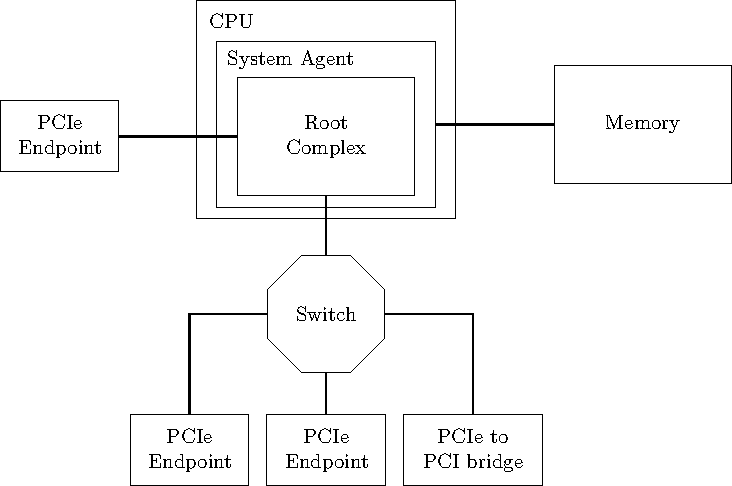
\includegraphics[width=0.6\textwidth]{figures/pcie-tree}
    \caption{Exemplary \acs{pcie} topology on an Intel system.}
    \label{fig:pcie-topology}
\end{figure}

Between \ac{pcie} devices and processor, switches may be used.
\Cref{fig:pcie-topology} depicts a typical \ac{pcie} tree. On the \ac{cpu} side,
connections end in the \ac{pcie} root complex which is part of the system agent
on Intel systems and the bridge between \ac{cpu}, main memory and devices. On
the device side, connections end at \ac{pcie} endpoints. \ac{pcie} devices may
initiate transfers to main memory through the \ac{pcie} root complex, acting as
\acs{dma} bus masters that access main memory independently of the \ac{cpu}.

\ac{pcie} uses three layers for communication: a physical layer, a data link
layer and a transaction layer. The physical layer of \ac{pcie} is responsible
for link initialization and point-to-point data transfer. The data link layer
ensures reliable transport of data between individual \ac{pcie} endpoints, or
endpoints and the root complex. The transaction layer contains user application
data or configuration data for the link, and routing information like
transmitter and receiver IDs for memory or \ac{io} requests.

Every \ac{pcie} transmission consists of four bytes that mark the start of a new
packet, a header of \SI{12}{\byte} (or 16 when using 64-bit addresses), a
payload of up to \SI{4096}{\byte} (depending on the maximum payload size on the
link), and 4 to \SI{8}{\byte} of packet checksums. Thus, the minimal packet
overhead for headers, checksums, etc. is \SI{20}{\byte}.

\ac{pcie} packets are categorized into requests and completions. Requests are
memory, \ac{io} or configuration reads and writes (to the PCI configuration
space) that are either posted, i.e., expect a completion (reply), or non-posted.
The PCI configuration space is a standardized register space that contains
information about a PCI(e) device such as vendor and device ID, device class or
the physical addresses of the device's registers (i.e., the Base Address
Registers or BARs). Among others, memory space is used by a device to access
main memory and by the \ac{cpu} to access device registers. \ac{io} space is
included for backwards compatibility and will probably be deprecated in the
future.

Device registers can be accessed via memory-mapped \ac{io} or port-mapped
\ac{io}. With memory-mapped \ac{io}, main memory and \ac{io} devices share the
same address space, i.e., all physical addresses refer to devices or main
memory. With port-mapped \ac{io}, special \ac{cpu} instructions and an \ac{io}
pin on the \ac{cpu} or a separate \ac{io} bus are used to perform \ac{io}.

To access the configuration space of \ac{pcie} devices, addresses consisting of
an eight bit bus number, five bit device number and three bit function number
are used (commonly referred to as BDF, i.e., bus/device/function). See
\Cref{fig:pcie-bdf} for reference. \ac{pcie} also specifies an ``Alternative
Routing-ID'' format where the 16-bit \ac{pcie} ID is split in an 8-bit bus
number and an 8-bit function number, i.e., device and function number merge into
one. However, this scheme does not yet seem to be used in practice
\cite[p.~24]{rothwell2018exploitation}.

\begin{figure}
    \centering
    \begin{bytefield}[endianness=big,bitwidth=0.03\linewidth]{16}
        \bitheader{0-15} \\
        \bitbox{8}{Bus \#} & \bitbox{5}{Device \#} & \bitbox{3}{Fn \#}
    \end{bytefield}
    \caption{\acs{pcie} IDs as bus/device/function triple.}
    \label{fig:pcie-bdf}
\end{figure}

On system boot, every \ac{pcie} root complex is enumerated to determine which
slots have devices installed. During enumeration, the \acs{bios}/\acs{uefi} or
\ac{os} probe the \ac{pcie} configuration space for all possible combinations of
bus and device number, i.e., by reading vendor and device ID of \ac{pcie}
switches and endpoints. It suffices to probe for function 0 for every
combination of bus and device number to determine a device's presence since
every device is required to implement function 0. For every detected device, the
maximum payload size on the link is determined and the device is assigned its
respective BDF. Bus and device numbers might be re-assigned by the enumeration
software if a \ac{pcie} device is hotplugged.

After a device's presence has been detected, every base address register field
in the configuration space is read to determine the address space needed to
access the registers of the device and subsequently every device is assigned a
portion of the host physical address space. If software sets one of the device's
registers through memory-mapped \ac{io}, e.g., during device setup by a device
driver, a memory write to the physical address is issued. The \ac{pcie} root
complex -- which unites the physical address space of all its devices --
receives the memory write, translates the physical address to the BDF of the
respective device and initiates a \ac{pcie} memory write transaction to the
device.


\section{Network Interface Controllers}
\label{sec:nics}

A common kind of \ac{pcie} peripherals are network cards used for communication
between computer systems via wireless (e.g., WLAN) or wired (e.g., LAN)
networks, often connecting hosts via a gateway to the Internet. Another term for
network card is \acf{nic}.

\begin{figure}[!b]
    \centering
    \includegraphics[width=0.4\textwidth]{figures/tx-ring}
    \caption{TX descriptor ring of a Network Interface Controller.}
    \label{fig:tx-ring}
\end{figure}

Manufacturers produce \acp{nic} for a wide range of applications, be it for data
centers with high performance requirements, or mobile phones and desktop
computers of the consumer sector. As versatile as these \acp{nic} are, so are
their drivers, and complexity of drivers and devices has increased over the
years: whereas early \acp{nic} were solely capable of receiving and transmitting
network packets, modern network cards offer plenty of (hardware-offloading)
features like checksum calculations, encryption and authentication of packets,
VLAN tagging and flow control, time syncing, traffic shaping, etc.

Complexity of \acp{nic} and drivers is reflected in several ways. On the one
hand in manuals (the datasheet for network cards of the Intel 82599 family
\cite{intel2019datasheet} consists of more than 1,000 pages) and driver size
(exceeding 100,000 lines of code for some devices \cite{emmerich2019case}). On
the other hand in devices like Intel's XL710 which follow a more firmware-driven
design where much functionality is executed on the network card, and driver and
\ac{nic} communicate via a message based interface \cite{emmerich2019user}. The
downside of this complexity in the currently dominant monolithic \aclp{os} is a
lack of reliability, safety and security: in case of Linux, 39 out of 40 memory
bugs found in the kernel in 2017 were located in device drivers
\cite{emmerich2019case}.

Although \acp{nic} have changed a lot in the last decades, most of them still
use a seemingly simplistic interface to communicate reception or transmittal of
packets: descriptor rings. Descriptor rings are circular buffers that contain
information about network packets and are shared between \ac{nic} and host.
\acp{nic} that use descriptor rings have RX and TX descriptor rings.
\Cref{fig:tx-ring} shows a TX descriptor ring. Descriptors in TX descriptor
rings describe outgoing packets, i.e., the amount of data to be sent, location
in memory (e.g., of buffers in a memory pool), whether transmittal of the packet
should be reported by the \ac{nic} through updating its descriptor, etc.
Conversely, descriptors in RX descriptor rings describe where incoming packets
can be stored by the \ac{nic}.

Ownership of descriptor rings is shared between \ac{nic} and host through two
queue pointers, a head and a tail pointer. In case of the TX descriptor ring,
the \ac{nic} manages the head pointer (TDH) while the device driver manages the
tail pointer (TDT). At device initialization, head and tail pointer are set to
the first descriptor. Once a packet is queued by the driver, i.e., the
descriptor in the TX descriptor ring has been changed appropriately, the driver
updates the tail pointer to the next descriptor, thereby transferring ownership
of all descriptors between head and tail pointer to the \ac{nic}. Conversely,
the \ac{nic} updates the head pointer once a descriptor was processed and the
corresponding packet data has been fetched from main memory by the \ac{nic}.

If the tail pointer points to the descriptor preceding the head pointer's
descriptor, the TX queue is full and no new data can be queued for transmittal.
Consequently, the driver has to wait until some packets have been sent out by
the \ac{nic}.


\section{Direct Memory Access}
\label{sec:dma}

Access to main memory by hardware without \ac{cpu} involvement is known as
\acf{dma}. By bypassing the \ac{cpu}, expensive memory operations can be
offloaded, potentially improving performance as the \ac{cpu} is no longer
involved in all memory transactions and therefore able to perform other
operations while data from/to main memory is transferred. In multi-core
processors, \ac{dma} is sometimes used to transfer data between cores. In
conjunction with \ac{pcie} devices, \ac{dma} is performed through \ac{pcie}
memory read and write transactions.

Using \ac{pcie}, no separate \ac{dma} controller is needed (third-party
\ac{dma}), instead reads and writes are issued directly from bus masters
(first-party \ac{dma}), i.e., \ac{pcie} devices allowed to read/write memory or
\ac{io} space. Memory reads and writes of main memory travel up the \ac{pcie}
tree to the root complex and subsequently to main memory via the memory
controller. Typically, physical addresses are used to access main memory in the
same way they are used by the \ac{cpu} when accessing device registers through
memory-mapped \ac{io}. However, use of physical addresses is troublesome as
\ac{pcie} devices may read from or write to any memory address of main memory,
which is a problem for

\begin{itemize}
    \item device pass-through to virtual machines, since virtual machines might
        read host memory outside of their access range through the memory
        accessing capabilities of \ac{pcie} devices;
    \item legacy 32-bit devices on 64-bit hosts, since they cannot access memory
        outside of their address space -- i.e., the first 4 GiB of host physical
        address space -- without bounce buffers and expensive memory copying by
        the \ac{os};
    \item avoiding harm from malicious or faulty drivers, since secrets can be
        read from main memory and \ac{os} data structures can be corrupted;
    \item avoiding harm from malicious or faulty devices;
    \item providing secure unprivileged access to hardware, e.g., in case of
        user-space network drivers.
\end{itemize}

To solve these problems, virtual addresses are used for \ac{io} devices on
modern computer systems instead of physical addresses. Similar to process
virtual addresses and \acp{mmu}, \acp{iova} are assigned to devices and a
translation unit is inserted into the data path that restricts memory accesses
to a device's memory region. Such translation units are commonly known as
\acfp{iommu}.


\section{Input-Output Memory Management Units}
\label{sec:iommus}

\acp{iommu} are multipurpose devices that primarily virtualize the memory space
of peripherals and provide interrupt remapping. Although there is a trend to use
\acp{iommu} as a protection mechanism against malicious or faulty peripherals,
the primary application for \acp{iommu} is and remains virtualization, i.e.,
direct pass-through of \ac{io} devices to virtual machines for higher throughput
and lower latency.

Conceptually, \acp{iommu} may be used for any kind of \ac{io} devices and any
kind of connection standard. In practice, \acp{iommu} are implemented in the
\ac{pcie} root complex since most if not all \ac{io} devices in today's systems
are connected to the \ac{cpu} via the \ac{pcie} root complex: modern interfaces
like Thunderbolt, NVMe and SATA Express are directly built on top of \ac{pcie},
and for older connection standards like USB or I$^2$C, \ac{pcie} hubs are used.
The focus of \acp{iommu} on \ac{pcie} is also reflected in code like Linux's
\ac{iommu} API that is closely centered around \ac{pcie} instead of providing an
abstract interface (e.g., focusing on \ac{pcie} BDF instead of generic groups).

Vendors use different marketing names for their \ac{iommu} solutions. Intel
calls it ``Intel Virtualization Technology for Directed I/O'' (VT-d), AMD uses
the term ``AMD I/O Virtualization Technology'' (AMD-V), and ARM does without
such a designation, simply denoting its \acp{iommu} as System Memory Management
Units (SMMUs).

In the VT-d specification, Intel describes different virtualization models for
\ac{io} devices, like direct assignment to virtual machines and \ac{io} device
sharing (see \ac{sriov} in \Cref{sec:sriov}), as well as the capabilities
provided by Intel VT-d required for these models, namely \ac{io} device
assignment, \ac{dma} remapping, interrupt remapping and ``reliability''
features. Besides virtualization, Intel also suggests some intra-\ac{os} use
cases for \ac{dma} remapping: protection of critical \ac{os} data from \ac{io}
devices, isolation of \ac{dma} accesses, support of high memory addresses for
legacy \ac{io} devices.

\ac{dma} remapping, i.e., address translation and access validation, is executed
by the remapping hardware inside of the \ac{iommu}. Intel calls this hardware
``DMA Remapping Hardware'', AMD uses the term ``I/O Virtualization Hardware'',
and ARM omits an additional term for this part of the hardware. In the following
paragraphs, we will use ``\acs{dmar} units'' when referring to the remapping
hardware.

\begin{figure} \centering
    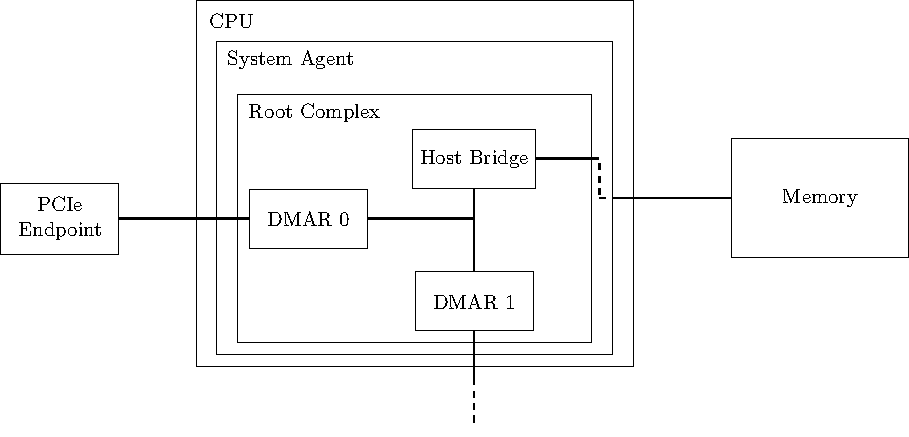
\includegraphics[width=0.7\textwidth]{figures/pcie-dmar}
    \caption{DMAR units in the PCIe root complex of an Intel system.}
    \label{fig:pcie-dmar}
\end{figure}

Every \ac{pcie} root complex may contain one or multiple \acp{iommu} where each
\ac{dmar} unit is responsible for a distinct set of \ac{io} buses
(\Cref{fig:pcie-dmar}). Devices on \ac{iommu}-managed buses belong to protection
domains, i.e., sets of address mappings and access permissions. While domains
may consist of multiple devices, devices belong to exactly one domain.

Data structures used for address translation by \ac{dmar} units are kept in main
memory to be accessible for \ac{os} and \acp{iommu}. In case of multiple
\acp{iommu}, \ac{dmar} units may share the same data structures. On \ac{iommu}
initialization, the \ac{os} sets up these data structures by creating domains
and address mappings for the system's \ac{io} devices. Although this happens at
system boot, mappings are not fix: the device-to-domain mapping may change
(e.g., when a device is assigned to a virtual machine) and address mappings may
be altered by the \ac{os} (e.g., when \ac{dma} memory is mapped or unmapped).

When \ac{io} devices attempt to access main memory, the request is intercepted
by the \ac{dmar} unit, checked for admissibility and translated appropriately.
This procedure consists of two major steps: First, a device's domain is
determined by its BDF number. Second, the domain's translation tables are
consulted to map the requested address to the host physical address, taking into
account the domain's translation scheme. Depending on the usage model of the
\ac{iommu}, the addresses used by \ac{io} devices may be one of the following:

\begin{itemize}
    \item \acp{iova} managed by software on the host,
    \item guest \acp{iova} managed by software in a virtual machine,
    \item guest physical addresses of a virtual machine,
    \item guest virtual addresses of software running in a virtual machine.
\end{itemize}

\begin{figure}[!b]
    \centering
    \includegraphics[width=1.0\textwidth]{figures/iova-translation}
    \caption{Intel \acs{iommu} address translation of 48-bit addresses to 4~KiB
    pages. Adapted from \cite{morgan2018iommu}.}
    \label{fig:translation}
\end{figure}

For different address types, hardware implementations of \acp{iommu} may support
different translation schemes. In case of virtualization, \acp{iommu} may be
used for nested translation of addresses: a first-level translation to translate
a guest virtual address to a guest physical address, followed by a second-level
translation translating the guest physical address to the host physical address.

\Cref{fig:translation} depicts the address translation mechanism of an Intel
\ac{iommu} for 48-bit \acp{iova} to 4 KiB pages. After an attempt to read or
write main memory has been intercepted by the \ac{iommu}, the first table to be
consulted -- if translation was enabled in the global command register of the
\ac{iommu} -- is the root table. The physical address of the root table is
stored in the Root Table Address Register (RTAR) of the \ac{iommu}. The root
table consists of 256 root entries \SI{16}{\byte} each, i.e., \SI{4}{\kibi\byte}
in total. Every root entry has a bit that indicates presence of a context table
for this entry. The root table is indexed by the bus number of the device and --
in conjunction with device and function number -- determines the context entry
for this device.

Like the root table, the context table is a \SI{4}{\kibi\byte} page with 256
\SI{16}{\byte} entries. Every context entry represents an \ac{iommu} domain.
Context entries contain a field indicating whether requests belonging to this
domain may pass the \ac{iommu} untranslated, and -- in the more likely case that
addresses must be translated -- a pointer to the first table to be used for
address translation for this domain, the PML4 table.

Subsequently, PML4, PDP, PD and the page table are walked by the \ac{iommu} to
determine the host physical address belonging to the \ac{iova}. Every table is a
\SI{4}{\kibi\byte} page with 512 \SI{8}{\byte} entries. If there is no
translation for a requested address or the access rights for the associated page
do not permit access, translation faults and the request is rejected.

In case of \SI{2}{\mebi\byte} pages, no PT table is used for translation, and
the last \SI{21}{\bit} of the \ac{iova} represent the offset into the
\SI{2}{\mebi\byte} page. In case of \SI{1}{\gibi\byte} pages, no PT and no PD
table are used, and the last \SI{30}{\bit} of the \ac{iova} represent the offset
into the \SI{1}{\gibi\byte} page. PML4, PDP, PD and PT table form a 4-level
translation structure. For 57-bit \acp{iova} and \SI{4}{\kibi\byte} pages, a
5-level structure is used with an additional PML5 table. For 39-bit \acp{iova}
and \SI{4}{\kibi\byte} pages, only three tables are used.

Intel's \ac{iommu} uses two different formats for the page table entries. For
first-level translation, entries equal the format used by the \ac{mmu} such that
the \ac{cpu} page tables can be re-used for address translation. For
second-level translation, a unique format is used.

AMD's \ac{iommu} is mostly identical to Intel's. One of the major differences is
that the AMD \ac{iommu} uses one table (called device table) to determine the
\ac{iommu} domain from the \ac{pcie} BDF identifier while Intel uses two, root
table and context table. With 65,536 possible BDF combinations, AMD's device
table consists of up to 65,536 entries with \SI{256}{\bit} each, i.e., up to
\SI{2}{\mebi\byte}. Another difference of AMD's \ac{iommu} is consistent usage
of the \ac{mmu} page table entries format for all translations.

ARM on the other hand uses a completely different design for its \ac{iommu}. Its
SMMUv2 specification describes a register-based architecture for small-scale
systems, and SMMUv3 with \ac{iommu} configuration stored in memory for larger
systems. The translation tables of these \acp{iommu} are compatible to the ARMv8
architecture. Like AMD's and Intel's \ac{iommu}, ARM determines the context of
the supplied address before address translation, however, context does not
depend on the BDF but a stream ID that is transmitted with every memory
transaction.

Common to all \acp{iommu} is caching of translation information in a context
cache and a \ac{tlb}, the \ac{iotlb}, to speed up address translation. While
context cache and \ac{iotlb} increase performance, they also increase complexity
as caches have to be kept up-to-date and entries must be purged from the caches
when they become invalid. If not implemented properly, this creates new
vulnerabilities as previous attacks have shown.


\section{IOMMUs on Linux}
\label{sec:iommus_on_linux}

Linux supports \acp{iommu} of all major vendors: besides Intel and AMD, the
kernel also includes drivers for \acp{iommu} from ARM, Qualcomm, Texas
Instruments, Samsung, Nvidia, IBM and other, less well-known manufacturers.

\acp{iommu} are not used by default on all architectures. In case of Intel x86,
Linux ignores any \ac{dmar} units and enables its own software \ac{iommu} called
SWIOTLB. The SWIOTLB is a poor man's \ac{iommu} that uses bounce buffers: At
boot time, a contiguous chunk of memory (usually \SI{64}{\mebi\byte}) is
reserved in the lower address space of main memory and used for \ac{dma}-capable
devices with limited addressing capabilities, e.g., legacy 32-bit devices. When
an already allocated \ac{dma} buffer is to be used by a device that cannot
address the buffer directly, memory in the lower address space, the so-called
aperture, is linked to that buffer, passed to the device, and data is copied
back and forth by the \ac{os} between the device-used memory in the aperture and
the device-inaccessible buffer.

On AMD systems, \acp{iommu} are enabled by default. For Intel, this behavior can
be enforced through a kernel boot parameter. When \acp{iommu} are enabled, Linux
checks the \acs{acpi} tables of \ac{bios}/\ac{uefi} for \ac{dmar} units on
system boot. For every DMA Remapping Hardware Unit Definition (DRHD) in the
\ac{dmar} reporting \ac{acpi} tables, Linux initializes the \ac{dmar} unit
through its respective device driver, creates a default \ac{iommu} domain and
assigns all \ac{pcie} devices to \ac{iommu} groups, where each group represents
the smallest possible set of devices that can be distinguished by the \ac{iommu}
(e.g., all devices behind a \ac{pcie}-to-PCI bridge belong to the same group).
Furthermore, each \ac{iommu} group is assigned to an \ac{iommu} domain.

Linux has a number of kernel boot parameters to change its default behavior in
relation to \acp{iommu}. (SW-)\acp{iommu} can be disabled or enforced, the
default domain can be set to pass-through such that devices bypass the
\ac{iommu} if not specified otherwise, and depending on the driver, the policy
of \ac{iotlb} management can be changed as Linux defers \ac{iotlb} invalidation
by default which increases performance but creates a window for invalid \ac{dma}
accesses, i.e., devices may access some \ac{dma}-able memory that has been
unmapped already as requests are still translated by the \ac{iotlb}. For the
Intel \ac{iommu}, \ac{iotlb} invalidation can be set to strict mode to enforce
immediate flushing of the \ac{iotlb}. The AMD \ac{iommu} driver provides a
similar option called \texttt{fullflush}. If no deviating behavior is specified,
Linux flushes the \acp{iotlb} every \SI{10}{\ms} or every 256 batched
invalidation requests.

Device drivers do not configure \acp{iommu} directly. Instead, they change the
\ac{iommu} configuration through Linux's \ac{dma}-API by allocating, mapping and
unmapping \ac{dma} memory, enforcing action by the respective \ac{iommu}
driver(s) depending on the operation and settings (e.g., immediate flushing of
all \acp{iotlb}).

\ac{dma}-mapping functions of the kernel return physical addresses as \ac{dma}
address when the \ac{pcie} device uses no \ac{iommu} and \acp{iova} with
\ac{iommu}. In both cases, memory is allocated using one of the kernel memory
allocator functions. Only in the second case, however, an \ac{iova} from the
device \ac{iommu} domain is allocated and the mapping from \ac{iova} to physical
address of the allocated memory is created through the \ac{iommu} driver.

For each \ac{iommu} domain, a base address and the upper boundary of
device-addressable \acp{iova} are assigned on initialization. Allocated
\acp{iova} are stored in a red-black tree which on allocation is searched for a
fitting address range bottom-up, i.e., from the highest \ac{iova} to the lowest.
To speed up \ac{iova} allocation, magazines are used, i.e., per core caches for
previously deallocated \acp{iova}.

For controlled device access in user-space, e.g., by user-space network drivers,
Linux offers a framework called \ac{vfio}. The framework consists of a device
driver and various \texttt{ioctl}s to interact with \ac{iommu}-controlled
\ac{pcie} devices.

Devices to be used through \ac{vfio} have to be bound to the \ac{vfio} device
driver. If a device's group contains multiple devices, all have to be bound to
the driver or must be unbound from other host drivers (which will make the group
available except the unbound devices). Device groups successfully bound to the
\ac{vfio} driver appear as files in Linux's device filesystem at
\texttt{/dev/vfio/\{group-number\}}. By chowning a device's group file to the
current user, unprivileged access to the \ac{pcie} devices of the group is
granted in a safe manner.

In \ac{vfio}, every \ac{iommu} group in use belongs to a container. Depending on
the \ac{iommu} driver's capabilities, one or multiple groups may be encapsulated
into a container, and containers may contain groups of different \ac{iommu}
domains.

To access a \ac{vfio}-bound device in user-space, multiple steps have to be
carried out by an application. The steps follow this scheme: First, a \ac{vfio}
container is created and initialized for the device to be used or an existing
container is re-used. Second, the device's group file is opened by the
user-space application and the group is added to the \ac{vfio} container. Third,
a file descriptor to the device is derived through a \ac{vfio} \texttt{ioctl}
call on the group file. Fourth, the device file descriptor is used to map the
device's registers into virtual memory. Finally, memory for \ac{dma} operations
may be allocated in user-space and \ac{iommu} mappings to that memory may be
created through the \ac{vfio}-API, returning \acp{iova} that can be passed to
the device.

Internally, \ac{vfio} stores its \ac{iova} mappings in a red-black tree.
Multiple mappings may be coalesced to reduce tracking overhead. When a new
mapping is requested through the \ac{vfio}-API, the red-black tree is checked
for overlapping mappings, validity of the requested \ac{iova} range is verified
(e.g., supported address width by affected \acp{iommu} vs. provided \ac{iova}
address width), the mapping is inserted into the tree, pages are pinned for
\ac{dma} access and the mapping is created in the \ac{iommu} tables via the
kernel-internal \ac{iommu}-API.


\section{Single-Root Input/Output Virtualization}
\label{sec:sriov}

% TODO: image physical function vs virtual function?

\Acf{sriov} is a mechanism that allows \ac{pcie} devices to appear as multiple
devices and thus be shared with multiple virtual machines. Devices that support
\ac{sriov} report this ability to the host via their PCI configuration space
which includes registers for \ac{sriov} Extended Capability.

When \ac{sriov} is enabled for a device, the device can be split into a \ac{pf}
and multiple \acp{vf}. The \ac{pf} is the standard \ac{pcie} function of the
device which has full control over the device, is used to reset and initialize
it and to enable and disable \acp{vf}. Hence, access to the \ac{pf} is usually
restricted to \ac{os} or virtual machine manager (VMM). \acp{vf} on the other
hand only support a subset of device operations, primarily to manage packet
receival and transmittal of the function, and can be passed to virtual machines
in a safe manner.

For \acp{vf}, separate drivers are used as \acp{vf} use different device
registers and have to communicate with the \ac{pf} driver for certain operations
like reset of the \ac{vf}. A \ac{pf} driver on the other hand must be able to
handle these requests and is hence slightly more complex than the same driver
without \ac{sriov} support.

On Linux, \acp{vf} of \ac{sriov}-capable devices can be created when loading the
\ac{pf} kernel driver, e.g., in case of \texttt{ixgbe}: \texttt{modprobe ixgbe
max\_vfs=2}, which results in the \ac{pf} driver creating two \acp{vf} for every
\texttt{ixgbe}-bound device in the system, or by writing the required number of
\acp{vf} into a device \texttt{sysfs} file called \texttt{sriov\_numvfs}.

When \acp{vf} are created by the \ac{pf} driver, every \ac{vf} is assigned a
\ac{pcie} BDF triple such that the \ac{vf} can be identified on the \ac{pcie}
bus and adressed directly. Although the function part of the BDF is only
\SI{3}{\bit}, i.e., eight different functions, more \acp{vf} can be created by
using different device numbers for the \acp{vf}.

Usually, the \ac{pf} also assigns MAC addresses to the \acp{vf} and configures
the \ac{nic} such that each \ac{vf} receives the packets destined to its MAC
address. To prevent MAC address spoofing, outgoing packets must be sent from the
\ac{vf}'s MAC address and are dropped by the \ac{nic} in case \acp{vf} do not
comply. The MAC anti-spoofing mechanism can be disabled by the \ac{pf} driver.

While not required, \ac{sriov} can be used in conjunction with \acp{iommu} to
pass \acp{vf} safely to virtual machines. When devices are passed-through
without \acp{iommu}, virtual machines have unlimited access to the machine's
main memory through the virtual function (see \Cref{sec:dma}).

